\documentclass{article}
\usepackage[utf8]{inputenc}
\usepackage[english]{babel}
\usepackage{graphicx}
\usepackage{pgfplots}
\begin{document}
\title{Usability of Web Browsers}
\author{Chris Dellomes\\
Professor: John Dionisio\\
CMSI 370: Interaction Design\\
	Loyola Marymount University}

\date{September 24, 2015}

\maketitle

\begin{center}
\begin{abstract}
\noindent This study is in response to the escalating competitive nature of the modern technology market. Usability is an ever growing factor in the success of software, necessitating usability tests. This paper presents comparative empirical evaluations involving two competing web browsers: Safari and Opera. Test participants were given three tasks to perform twice on each web browser. The results of this evaluation include (a) testing factors during the study, (b) quantitative data collected during testing, and (c) usability metrics measured. This paper incorporates the data gathered into a heuristic evaluation of each web browser.
\end{abstract}


\bigskip

\textit{Group Members}: Peyton Cross, Irakli Khizanishvili, Mary Kate Reid
\end{center}

\thispagestyle{empty}

\clearpage

\setcounter{page}{1}

\section{Introduction} When Apple unveiled the Safari web browser back in 2003, it was advertised as the fastest web browser for the Macintosh and including a multitude of innovative features, such as a bookmark library. Originally exclusive to Apple computers, Safari later became available in 2007 for Windows until it was discontinued in 2012. Though not currently the most popular browser, it is currently the default web browser on iOS and OS X, with approximately 16\% of individuals globally using it as their preferred browser. Preceding Safari, Opera was originally a research project by Telenor until it became its own entity and publicly released in 1995. Users originally had to purchase Opera, until it moved to an advertisement based system which lasted from 2000 to 2005. Since its release, less than 5\% of web browser users worldwide used Opera as their preferred web browser, making it a relatively unpopular browser. While Safari is noticeably more widely used than Opera, they are comparable in terms of features.\\
\\
\indent Though neither browser is currently the most popular, it is still important to address the usability of each since Safari and Opera are still widely used worldwide. This study uses empirically examines the usability of each web browser. Within the Interaction Design field, usability is based on five distinct metrics: learnability, efficiency, errors, memorability, and satisfaction. This study will primarily focus on learnability, efficiency, and errors.

\section{Testing Factors} Before each test subject performed the assigned tasks, users were asked how much experience they had in using each web browser. Finding test subjects who had little to no prior experience with both web browsers was relatively simple. Since this study focused on both learnability and efficiency, we tested subjects when they were inexperienced with both browsers and again when they had ample experience performing the tasks.

\section{Testing Procedures} Each test subject performed three distinct tasks on each browser. They were tested when they had little to no experience to the browser, allowed to practice performing the tasks, then tested again once they felt comfortable performing the tasks.
\begin{enumerate}
	\item Change the home page of the web browser.
	\item Bookmark a webpage.
	\item Use the history to find and access a webpage visited the previous day.
\end{enumerate}
To keep the testing controlled, each subject was tested on a computer running OS X. As study participants performed each task, information regarding their learnability, efficiency, and errors were collected.

\subsection{Learnability}
\par
\textbf{First Task: } Change the home page of the web browser.
\begin{center}
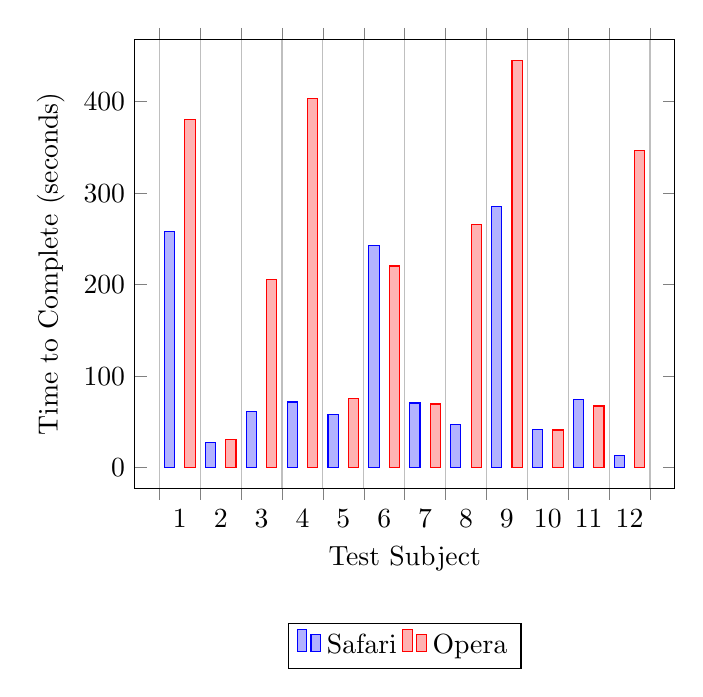
\begin{tikzpicture}
\begin{axis}[
	x tick label style={
		/pgf/number format/1000 sep=},
	xlabel= Test Subject,
	ylabel=Time to Complete (seconds),
	enlargelimits=0.05,
	legend style={at={(0.5,-0.3)},
	anchor=north,legend columns=-1},
	ybar interval=0.5,
]
\addplot 
	coordinates {(1, 258.1) (2, 27.6) (3, 61.5) (4, 71.8) (5, 57.8) (6, 243.0) (7, 70.7) (8, 46.8) (9, 285.2) (10, 41.7) (11, 74.9) (12, 13.1) (13, 0)};
\addplot
	coordinates {(1, 381.0) (2, 30.7) (3, 205.7) (4, 403.0) (5, 75.6) (6, 220.4) (7, 69.6) (8, 265.4) (9, 445.4) (10, 41.2) (11, 67.4) (12, 346.2) (13, 0)};
\legend{Safari,Opera}
\end{axis}
\end{tikzpicture}

\par Average time for Learnability task \#1 on Safari: \textit{104.4 seconds}
\par Average time for Learnability task \#1 on Opera: \textit{212.6 seconds}
\end{center}
\par \noindent The results of this task indicate that on average, it is significantly easier to learn how to change the home page in Safari.

\clearpage

\par
\textbf{Second Task: } Bookmark a webpage.
\begin{center}
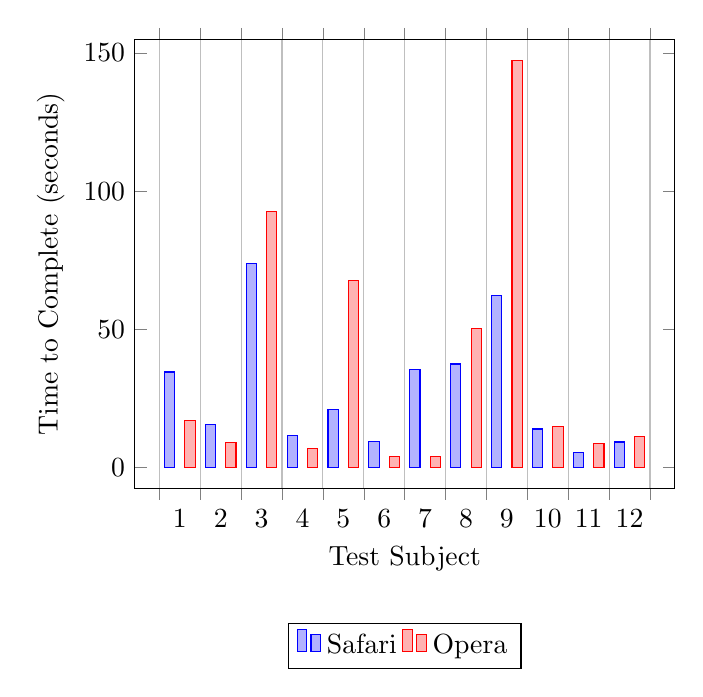
\begin{tikzpicture}
\begin{axis}[
	x tick label style={
		/pgf/number format/1000 sep=},
	xlabel= Test Subject,
	ylabel=Time to Complete (seconds),
	enlargelimits=0.05,
	legend style={at={(0.5,-0.3)},
	anchor=north,legend columns=-1},
	ybar interval=0.5,
]
\addplot 
	coordinates {(1, 34.6) (2, 15.6) (3, 73.7) (4, 11.7) (5, 21.2) (6, 9.4) (7, 35.4) (8, 37.5) (9, 62.2) (10, 14.0) (11, 5.6) (12, 9.3) (13, 0)};
\addplot
	coordinates {(1, 17.1) (2, 9.1) (3, 92.8) (4, 6.8) (5, 67.7) (6, 3.9) (7, 4.0) (8, 50.2) (9, 147.4) (10, 14.9) (11, 8.8) (12, 11.2) (13, 0)};
\legend{Safari,Opera}
\end{axis}
\end{tikzpicture}

\par Average time for Learnability task \#2 on Safari: \textit{27.5 seconds}
\par Average time for Learnability task \#2 on Opera: \textit{36.2 seconds}
\end{center}
\par \noindent The results of this task indicate that on average, it is easier to learn how to bookmark a page in Safari.

\clearpage

\par
\textbf{Third Task: } Use the history to find and access a webpage visited the previous day.
\begin{center}
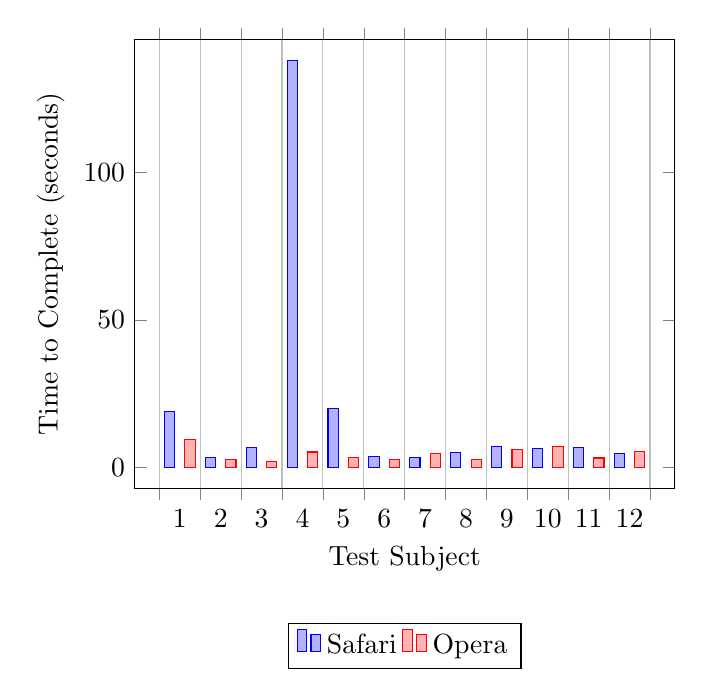
\begin{tikzpicture}
\begin{axis}[
	x tick label style={
		/pgf/number format/1000 sep=},
	xlabel= Test Subject,
	ylabel=Time to Complete (seconds),
	enlargelimits=0.05,
	legend style={at={(0.5,-0.3)},
	anchor=north,legend columns=-1},
	ybar interval=0.5,
]
\addplot 
	coordinates {(1, 19.1) (2, 3.5) (3, 6.8) (4, 138.0) (5, 20.1) (6, 3.9) (7, 3.5) (8, 5.2) (9, 7.1) (10, 6.5) (11, 6.9) (12, 4.9) (13, 0)};
\addplot
	coordinates {(1, 9.7) (2, 2.8) (3, 2.2) (4, 5.3) (5, 3.5) (6, 2.7) (7, 4.9) (8, 2.7) (9, 6.3) (10, 7.3) (11, 3.3) (12, 5.4) (13, 0)};
\legend{Safari,Opera}
\end{axis}
\end{tikzpicture}

\par Average time for Learnability task \#3 on Safari: \textit{18.8 seconds}
\par Average time for Learnability task \#3 on Opera: \textit{5.3 seconds}
\end{center}
\par \noindent The results of this task indicate that on average, it is slightly easier to learn how to access the histoey in Opera.\footnote{While users completed the task on Safari faster on average, it is important to note the outlier which significantly raised the average time.}

\clearpage

\subsection{Efficiency}
\par
\textbf{First Task: } Change the home page of the web browser.
\begin{center}
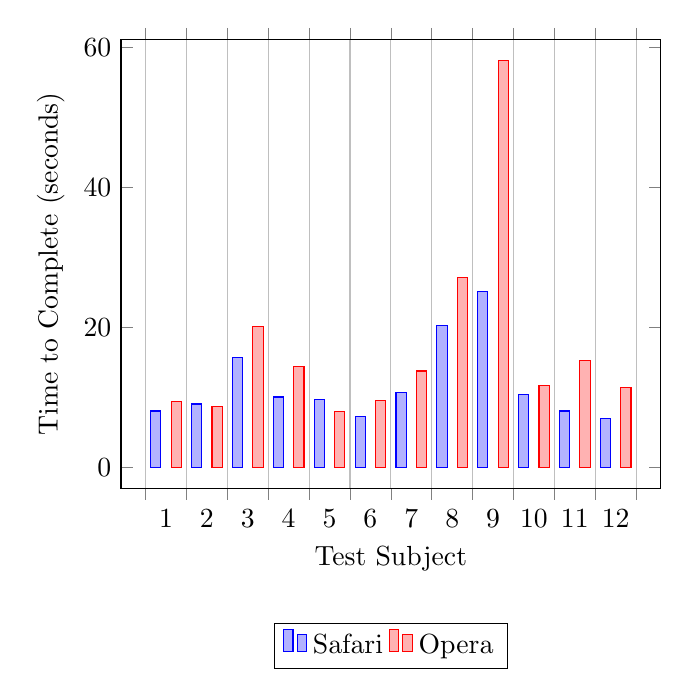
\begin{tikzpicture}
\begin{axis}[
	x tick label style={
		/pgf/number format/1000 sep=},
	xlabel= Test Subject,
	ylabel=Time to Complete (seconds),
	enlargelimits=0.05,
	legend style={at={(0.5,-0.3)},
	anchor=north,legend columns=-1},
	ybar interval=0.5,
]
\addplot 
	coordinates {(1, 8.1) (2, 9.1) (3, 15.7) (4, 10.1) (5, 9.8) (6, 7.3) (7, 10.7) (8, 20.3) (9, 25.1) (10, 10.4) (11, 8.1) (12, 7.0) (13, 0)};
\addplot
	coordinates {(1, 9.4) (2, 8.8) (3, 20.2) (4, 14.5) (5, 8.0) (6, 9.6) (7, 13.8) (8, 27.2) (9, 58.2) (10, 11.8) (11, 15.3) (12, 11.4) (13, 0)};
\legend{Safari,Opera}
\end{axis}
\end{tikzpicture}

\par Average time for Efficiency task \#1 on Safari: \textit{11.8 seconds}
\par Average time for Efficiency task \#1 on Opera: \textit{17.4 seconds}
\end{center}
\par \noindent The results of this task indicate that on average, users are more efficient at changing Safari's home page.

\clearpage

\par
\textbf{Second Task: } Bookmark a webpage.
\begin{center}
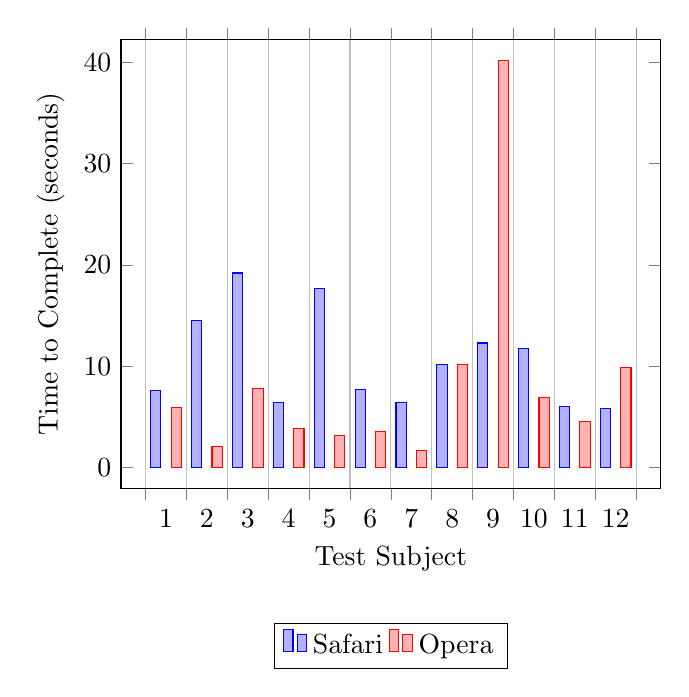
\begin{tikzpicture}
\begin{axis}[
	x tick label style={
		/pgf/number format/1000 sep=},
	xlabel= Test Subject,
	ylabel=Time to Complete (seconds),
	enlargelimits=0.05,
	legend style={at={(0.5,-0.3)},
	anchor=north,legend columns=-1},
	ybar interval=0.5,
]
\addplot 
	coordinates {(1, 7.6) (2, 14.5) (3, 19.2) (4, 6.4) (5, 17.7) (6, 7.7) (7, 6.4) (8, 10.2) (9, 12.3) (10, 11.8) (11, 6.0) (12, 5.8) (13, 0)};
\addplot
	coordinates {(1, 5.9) (2, 2.1) (3, 7.8) (4, 3.9) (5, 3.2) (6, 3.6) (7, 1.7) (8, 10.2) (9, 40.2) (10, 6.9) (11, 4.6) (12, 9.9) (13, 0)};
\legend{Safari,Opera}
\end{axis}
\end{tikzpicture}

\par Average time for Efficiency task \#2 on Safari: \textit{10.5 seconds}
\par Average time for Efficiency task \#2 on Opera: \textit{8.3 seconds}
\end{center}
\par \noindent The results of this task indicate that on average, users are more efficient at bookmarking webpages in Opera.

\clearpage

\par
\textbf{Third Task: } Use the history to find and access a webpage visited the previous day.
\begin{center}
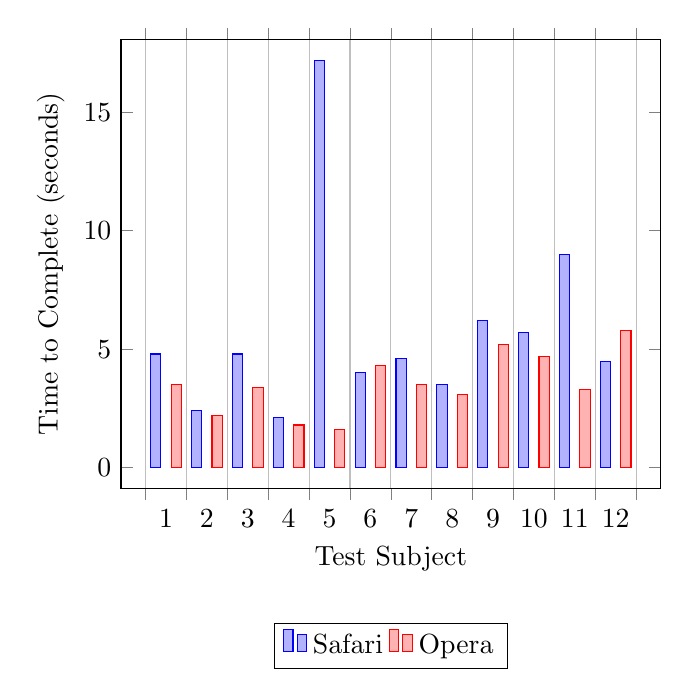
\begin{tikzpicture}
\begin{axis}[
	x tick label style={
		/pgf/number format/1000 sep=},
	xlabel= Test Subject,
	ylabel=Time to Complete (seconds),
	enlargelimits=0.05,
	legend style={at={(0.5,-0.3)},
	anchor=north,legend columns=-1},
	ybar interval=0.5,
]
\addplot 
	coordinates {(1, 4.8) (2, 2.4) (3, 4.8) (4, 2.1) (5, 17.2) (6, 4.0) (7, 4.6) (8, 3.5) (9, 6.2) (10, 5.7) (11, 9.0) (12, 4.5) (13, 0)};
\addplot
	coordinates {(1, 3.5) (2, 2.2) (3, 3.4) (4, 1.8) (5, 1.6) (6, 4.3) (7, 3.5) (8, 3.1) (9, 5.2) (10, 4.7) (11, 3.3) (12, 5.8) (13, 0)};
\legend{Safari,Opera}
\end{axis}
\end{tikzpicture}

\par Average time for Efficiency task \#3 on Safari: \textit{5.7 seconds}
\par Average time for Efficiency task \#3 on Opera: \textit{3.5 seconds}
\end{center}
\par \noindent The results of this task indicate that on average, users are more efficient at accessing the browsing history in Opera

\clearpage

\subsection{Errors}
\par The errors recorded during this study are as defined by Interaction Design conventions: instances where the user performs an action that results in an unexpected consequence. The following table provides some examples of errors common among study participants.

\begin{center}
\begin{table}[ht]
\begin{tabular}{l|c|c}
Task & Browser & Error\\ \hline
Task1 & Opera & Click button to add page to top sites instead of make homepage\\
Task1 & Safari & Click top sites button trying to access options\\
Task2 & Safari & Click the bookmarks / reading list button instead of adding bookmark
\end{tabular}
\end{table}

\medbreak

\textbf{First Task Errors: } Number of errors made during the first task.
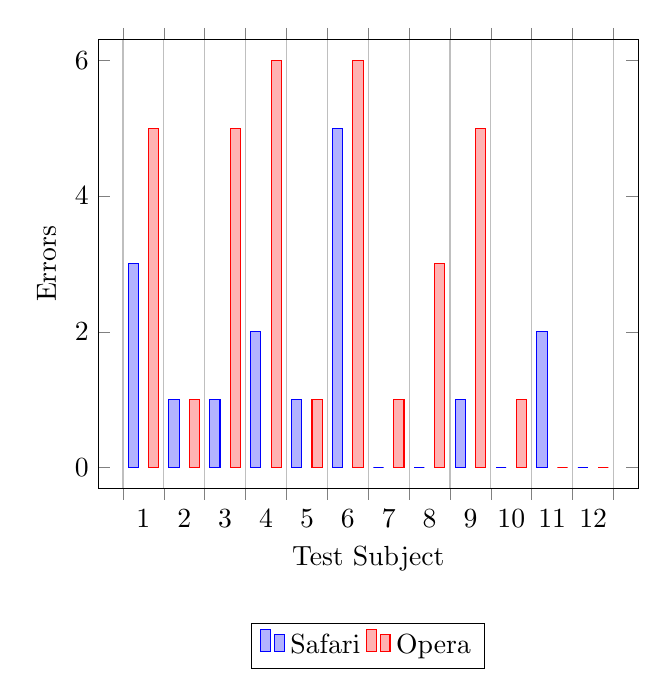
\begin{tikzpicture}
\begin{axis}[
	x tick label style={
		/pgf/number format/1000 sep=},
	xlabel= Test Subject,
	ylabel=Errors,
	enlargelimits=0.05,
	legend style={at={(0.5,-0.3)},
	anchor=north,legend columns=-1},
	ybar interval=0.5,
]
\addplot 
	coordinates {(1, 3) (2, 1) (3, 1) (4, 2) (5, 1) (6, 5) (7, 0) (8, 0) (9, 1) (10, 0) (11, 2) (12, 0) (13, 0)};
\addplot
	coordinates {(1, 5) (2, 1) (3, 5) (4, 6) (5, 1) (6, 6) (7, 1) (8, 3) (9, 5) (10, 1) (11, 0) (12, 0) (13, 0)};
\legend{Safari,Opera}
\end{axis}
\end{tikzpicture}

\par Average number of errors for task \#1 \textit{1.3 errors}
\par Average number of errors for task \#1 \textit{2.8 errors}
\end{center}
\par \noindent The results of this task indicate that users are less inclined to commit errors in Safari.

\clearpage

\textbf{Second Task Errors: } Number of errors made during the second task.
\begin{center}
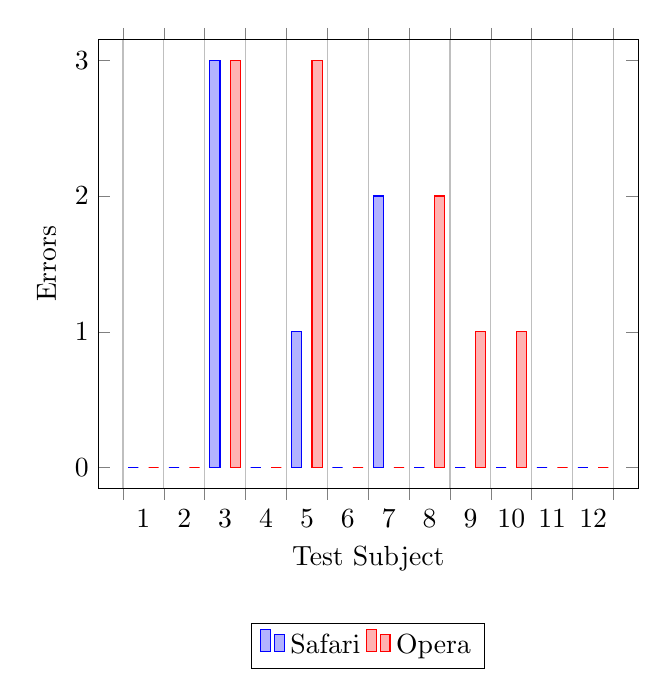
\begin{tikzpicture}
\begin{axis}[
	x tick label style={
		/pgf/number format/1000 sep=},
	xlabel= Test Subject,
	ylabel=Errors,
	enlargelimits=0.05,
	legend style={at={(0.5,-0.3)},
	anchor=north,legend columns=-1},
	ybar interval=0.5,
]
\addplot 
	coordinates {(1, 0) (2, 0) (3, 3) (4, 0) (5, 1) (6, 0) (7, 2) (8, 0) (9, 0) (10, 0) (11, 0) (12, 0) (13, 0)};
\addplot
	coordinates {(1, 0) (2, 0) (3, 3) (4, 0) (5, 3) (6, 0) (7, 0) (8, 2) (9, 1) (10, 1) (11, 0) (12, 0) (13, 0)};
\legend{Safari,Opera}
\end{axis}
\end{tikzpicture}

\par Average number of errors for task \#1 \textit{0.5 errors}
\par Average number of errors for task \#1 \textit{0.8 errors}
\end{center}
\par \noindent The results of this task indicate that users are slightly less inclined to commit errors in Safari.

\clearpage

\textbf{Third Task Errors: } Number of errors made during the second task.
\begin{center}
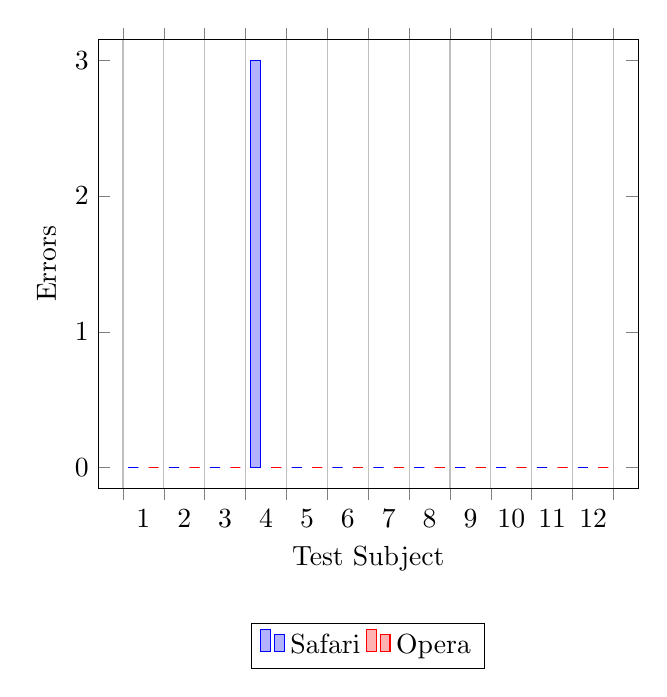
\begin{tikzpicture}
\begin{axis}[
	x tick label style={
		/pgf/number format/1000 sep=},
	xlabel= Test Subject,
	ylabel=Errors,
	enlargelimits=0.05,
	legend style={at={(0.5,-0.3)},
	anchor=north,legend columns=-1},
	ybar interval=0.5,
]
\addplot 
	coordinates {(1, 0) (2, 0) (3, 0) (4, 3) (5, 0) (6, 0) (7, 0) (8, 0) (9, 0) (10, 0) (11, 0) (12, 0) (13, 0)};
\addplot
	coordinates {(1, 0) (2, 0) (3, 0) (4, 0) (5, 0) (6, 0) (7, 0) (8, 0) (9, 0) (10, 0) (11, 0) (12, 0) (13, 0)};
\legend{Safari,Opera}
\end{axis}
\end{tikzpicture}

\par Average number of errors for task \#1 \textit{0.25 errors}
\par Average number of errors for task \#1 \textit{0 errors}
\end{center}
\par \noindent The results of this task indicate that, aside from outliers, users are unlikely to commit errors when accessing history.

\section{Heuristic Evaluation} Along with usability metrics, heuristic evaluation on why each system performed how they did is vital to understanding the usability of each web browser. This evaluation will be based on related guidelines and best practices documentation.

\subsection{Safari--- Icons} The Safari web browser utilizes a combination of menus at the top of the screen and icons within the browser page. The browser icons comply with Apple's OS X Human Interface Guidelines: simplistic and unique in structure. These practices are evident in the below screenshot, such as with the bookmarks sidebar icon indicated by the book icon. However, it and other icons are somewhat misleading in design, which led to several user errors. For example, the plus icon next to the address bar was mistaken for bookmarking the page, when it actually adds the page to the reading list, which is seperate from bookmarks. \clearpage \noindent Also, the plus icon at the bottom of the bookmarks sidebar was interpreted by multiple test participants to add a bookmark when in reality it created a new folder for bookmarks to be stored. Though the icons are simplistic and unique, they still mislead users in their intended consequences. Multiple users committed errors related to clicking incorrect or unrelated icons. It would be interesting if, in a future study, redesigning the icons or removing them entirely and having users focus on the menus would result in improved usability.
\begin{center}
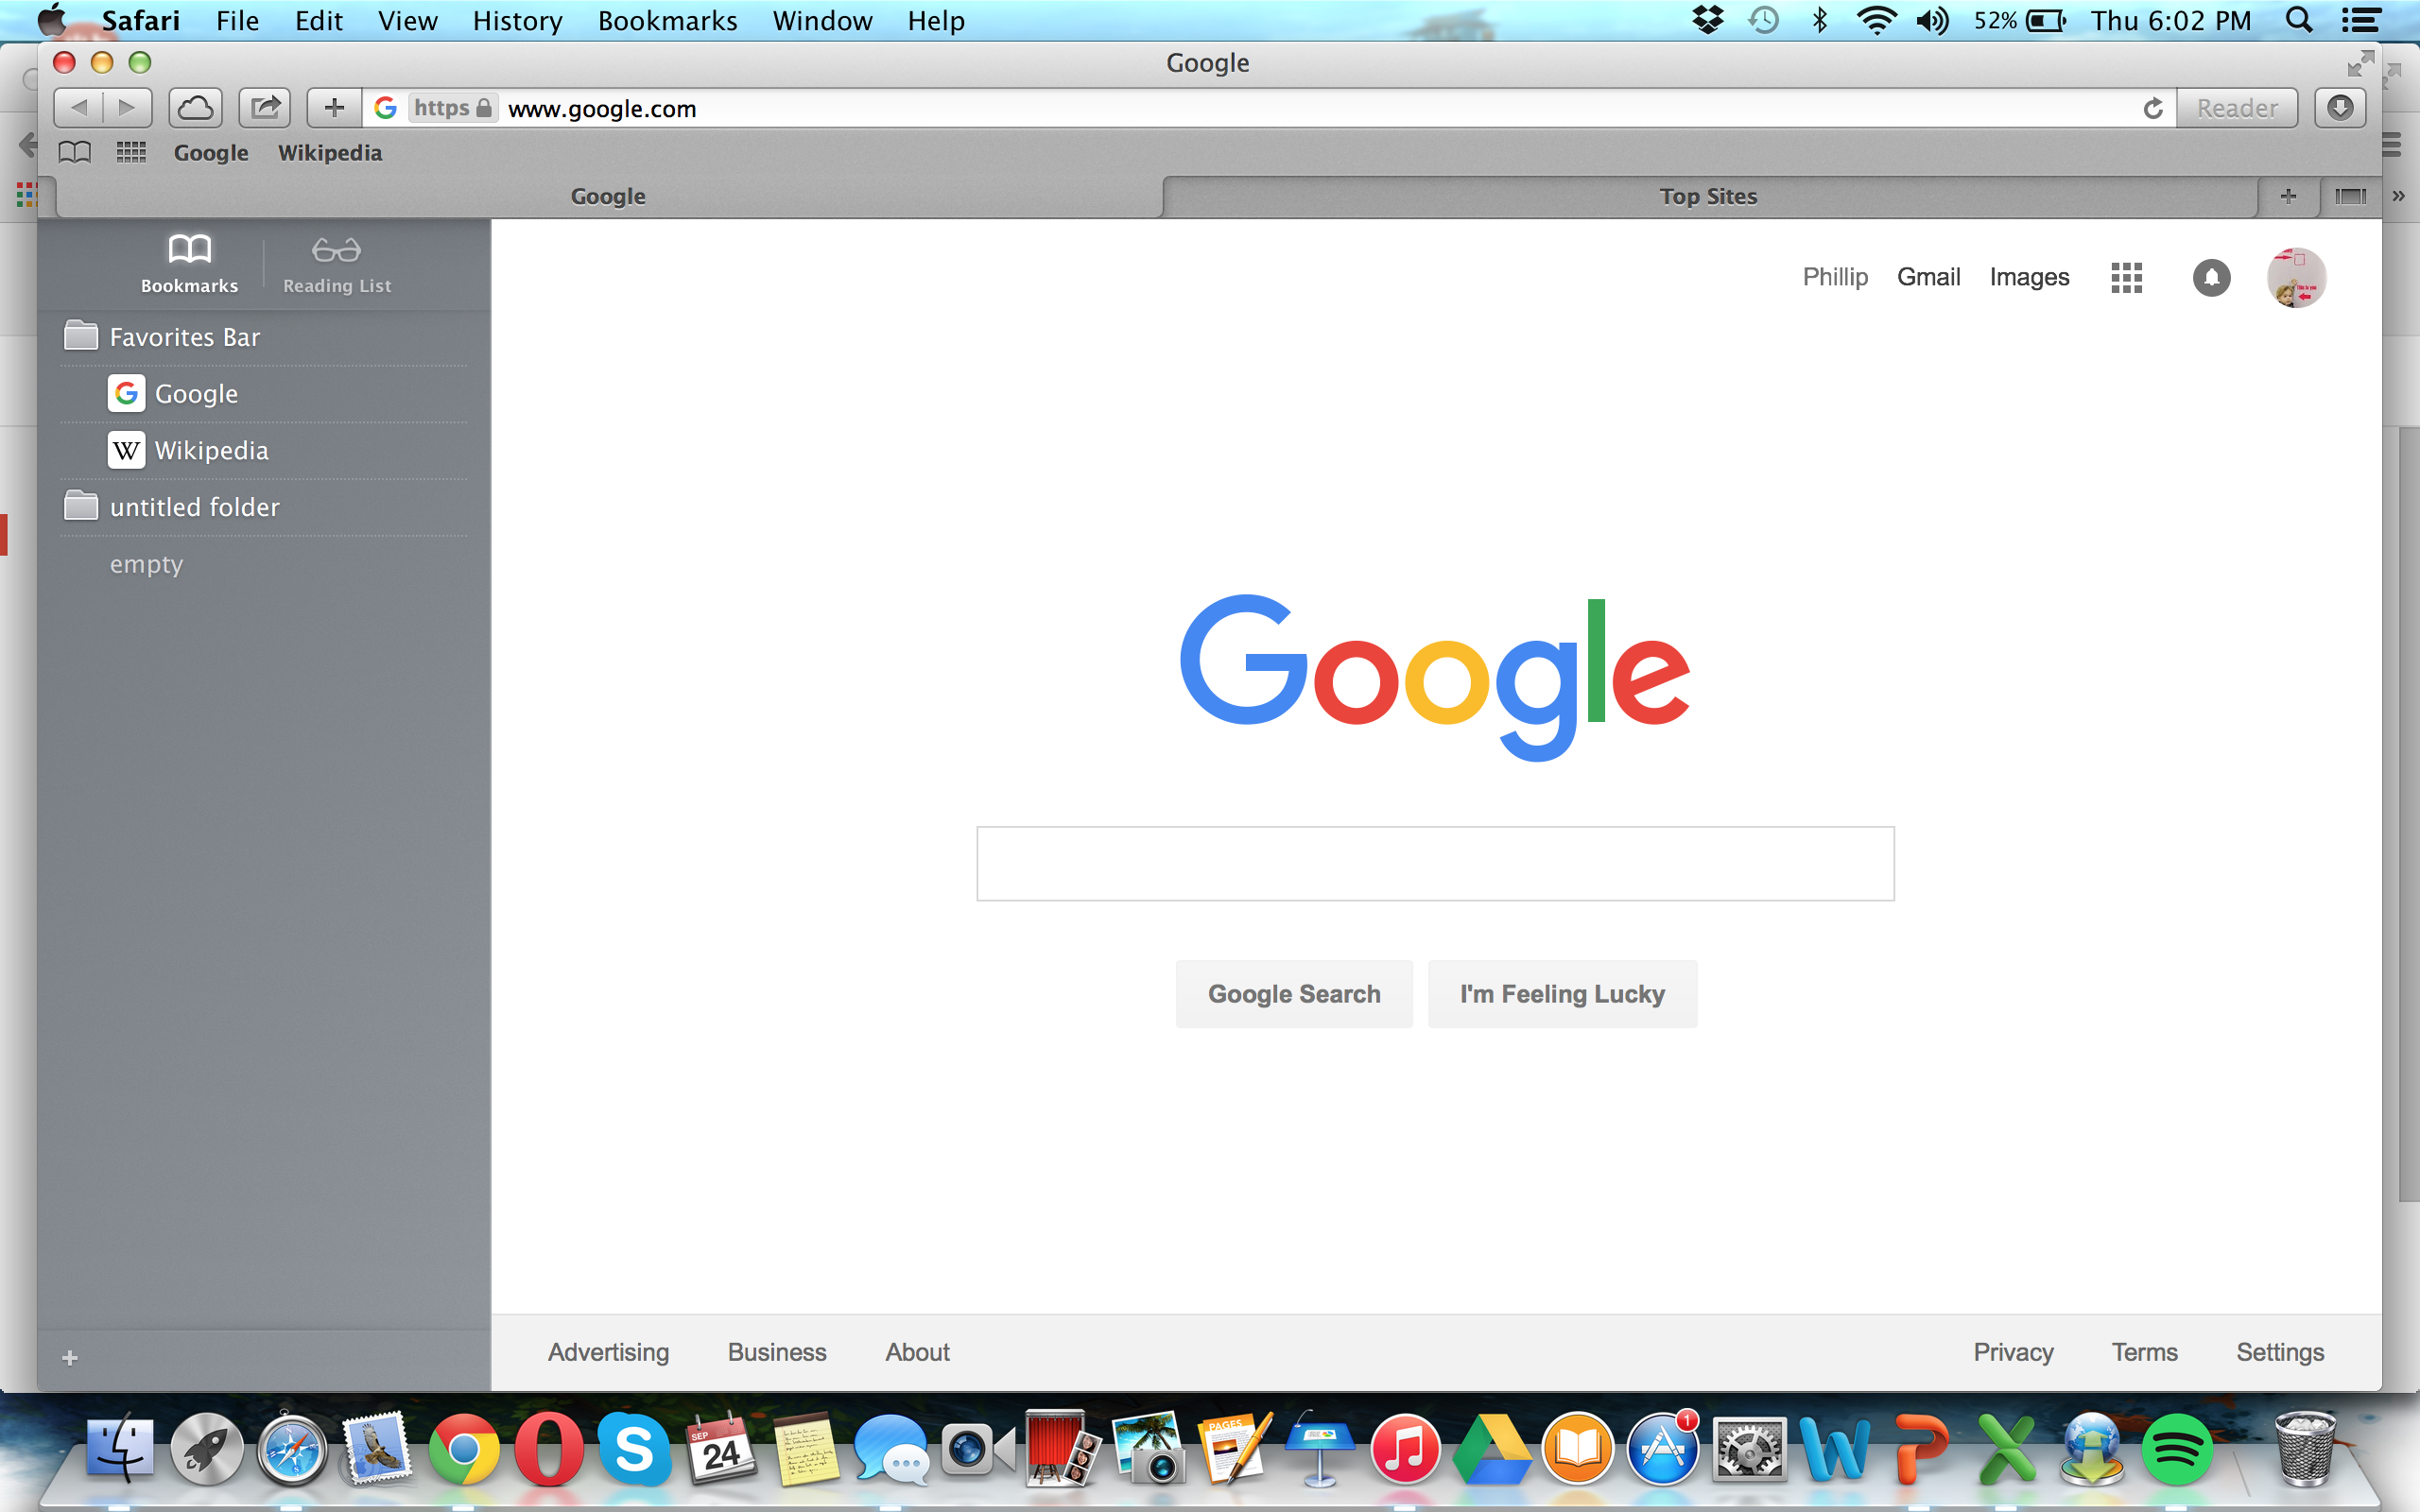
\includegraphics[width=1\textwidth]{Safari_Bookmark.png}
\end{center}

\subsection{Opera--- Menus} The Opera web browser utilizes similar menus to the Safari browser. Browser, history and homepage are access in the bookmarks, history, and preferences menus in both browsers. However, Opera's menus do not entirely comply with Apple's OS X Human Interface guidelines in that their menus do not always accurately and concisely represent menu items. This is evident with the preferences menu in the picture below, where users change their homepage. While Safari explicitly indicates where to change the homepage, Opera instead places the option within the on startup section. 
\begin{center}
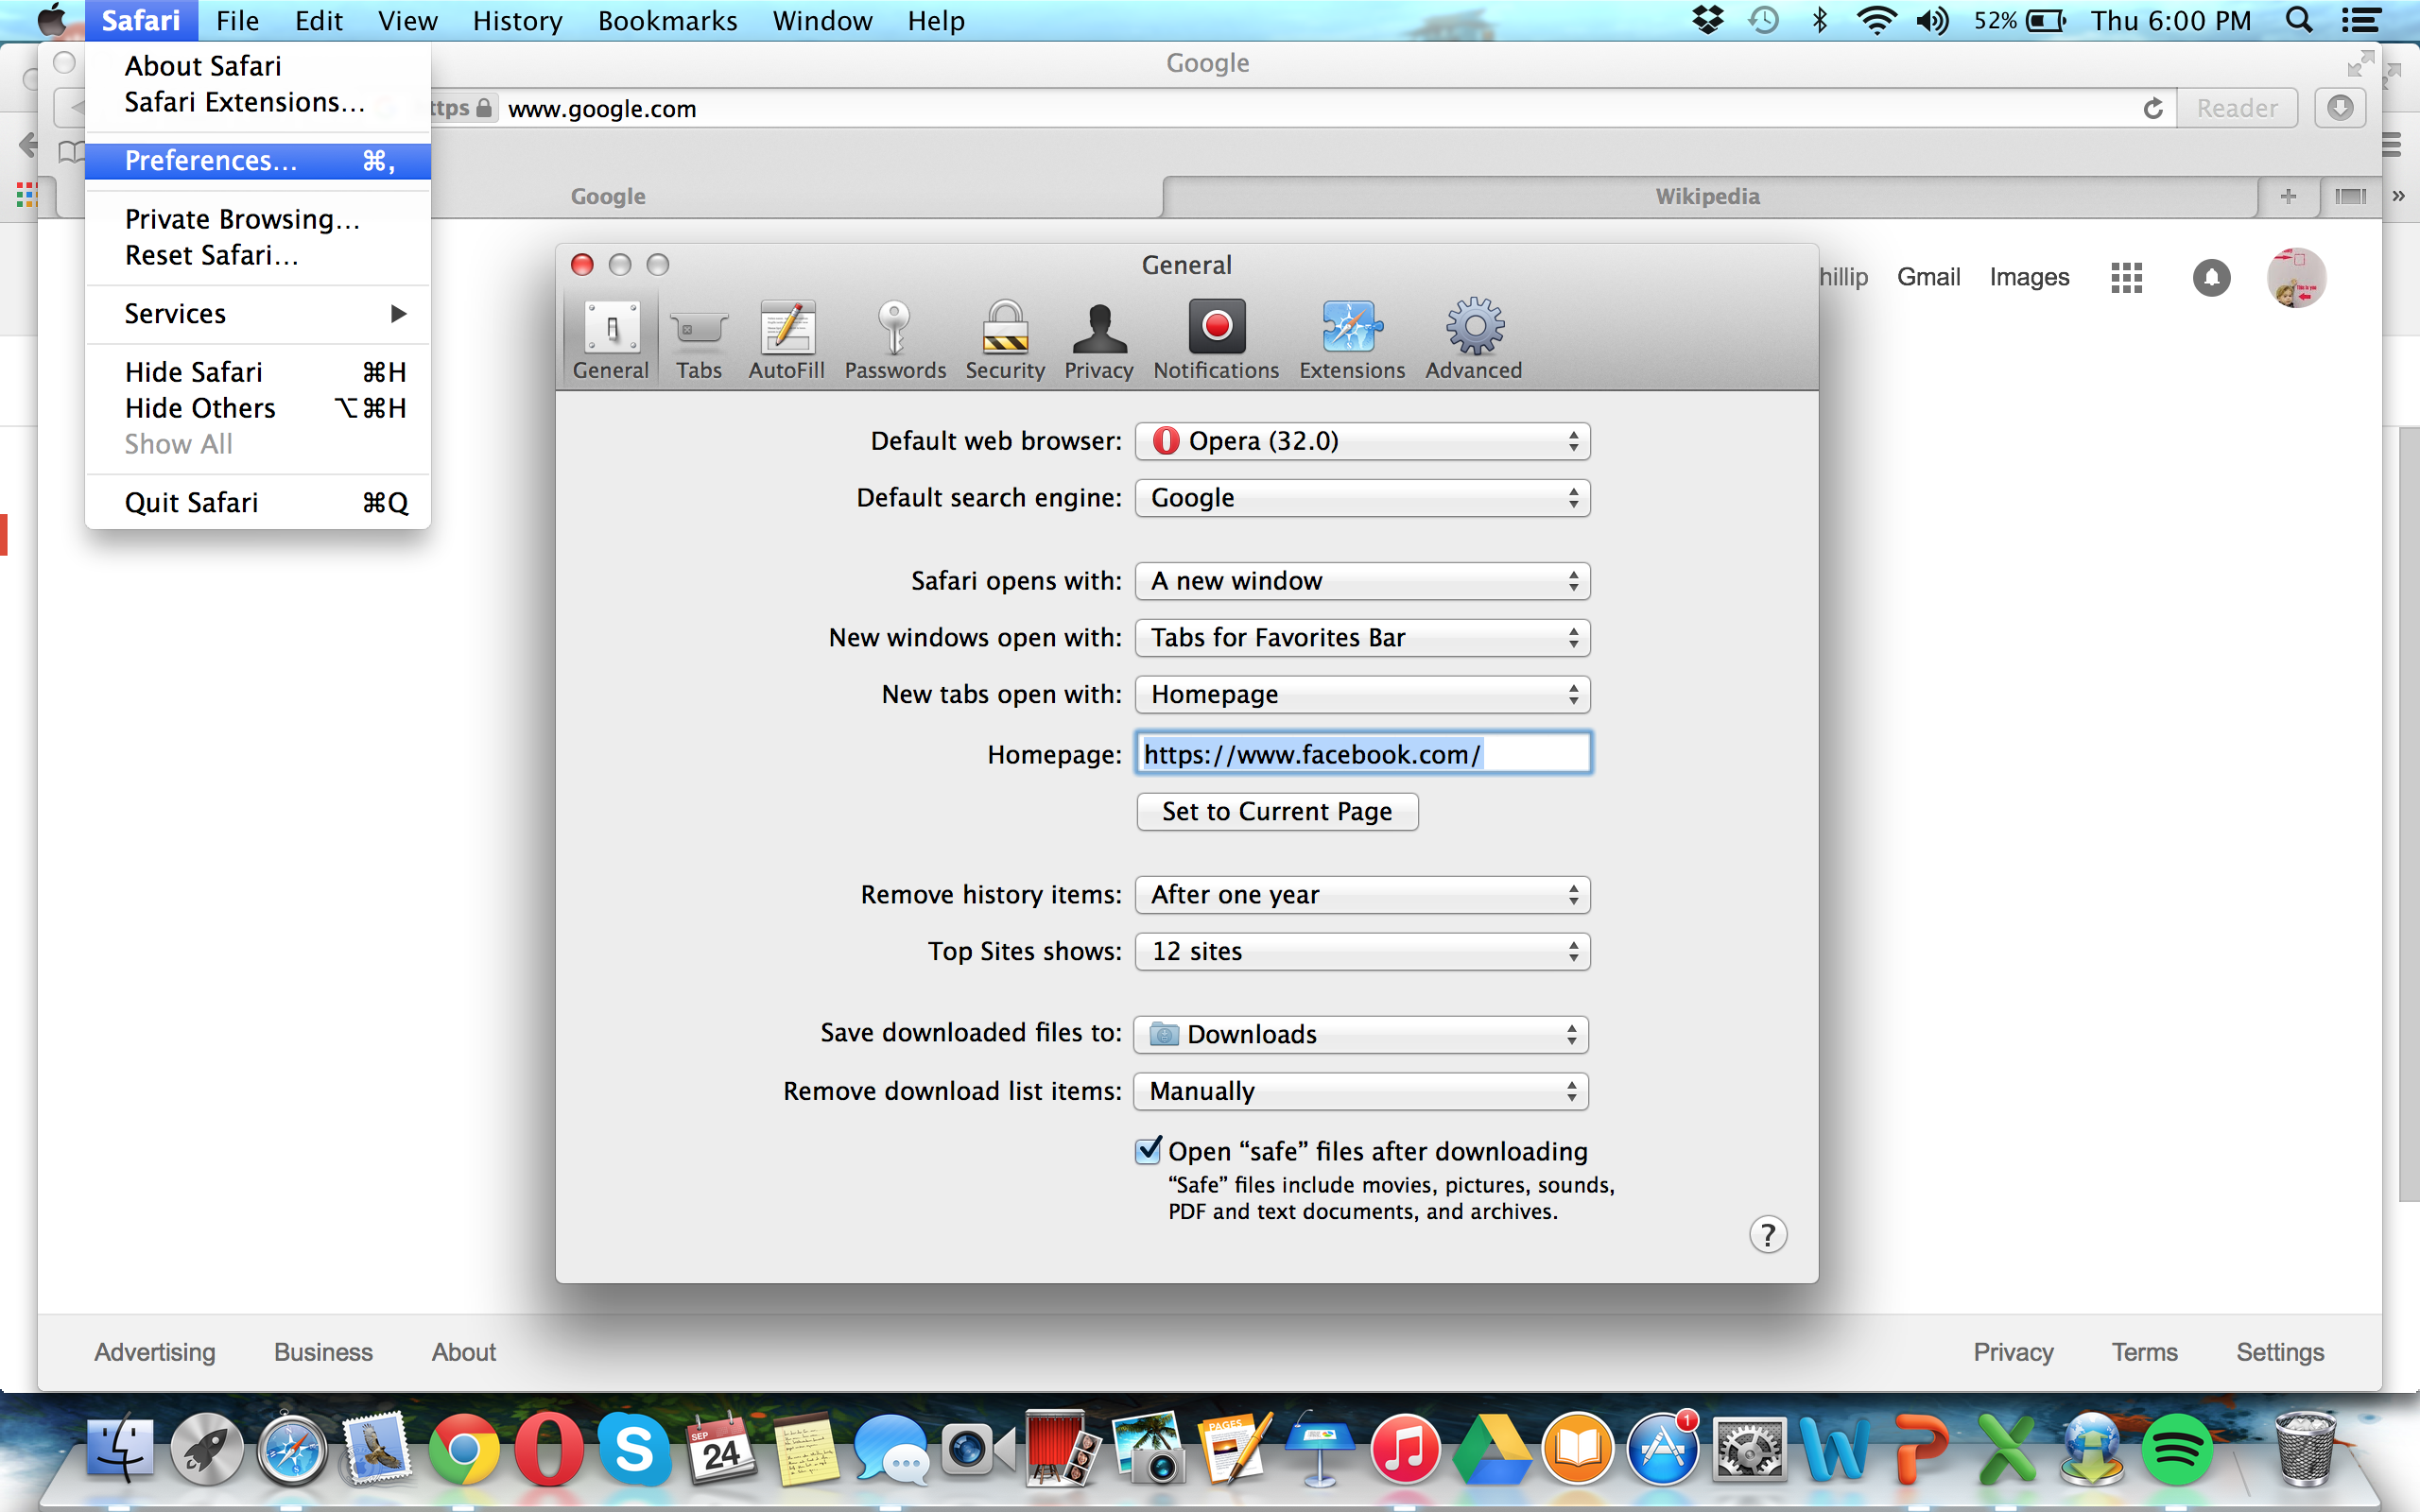
\includegraphics[width=1\textwidth]{Safari_Homepage.png}
\end{center}
Also, instead of explicitly saying homepage, Opera gives a blue link where users set pages. Because the homepage is not specifically mentioned in the preferences, many users made the mistake of browsing over the set pages option and navigating away from the preferences menu entirely. Though the developers of Opera utilize a similar mental model for accessing options, such as homepage and bookmarks, menu titles misrepresent menu items and result in reduced usability. There is potential for increasing Opera's usability by making menu names more concise and accurate.
\begin{center}
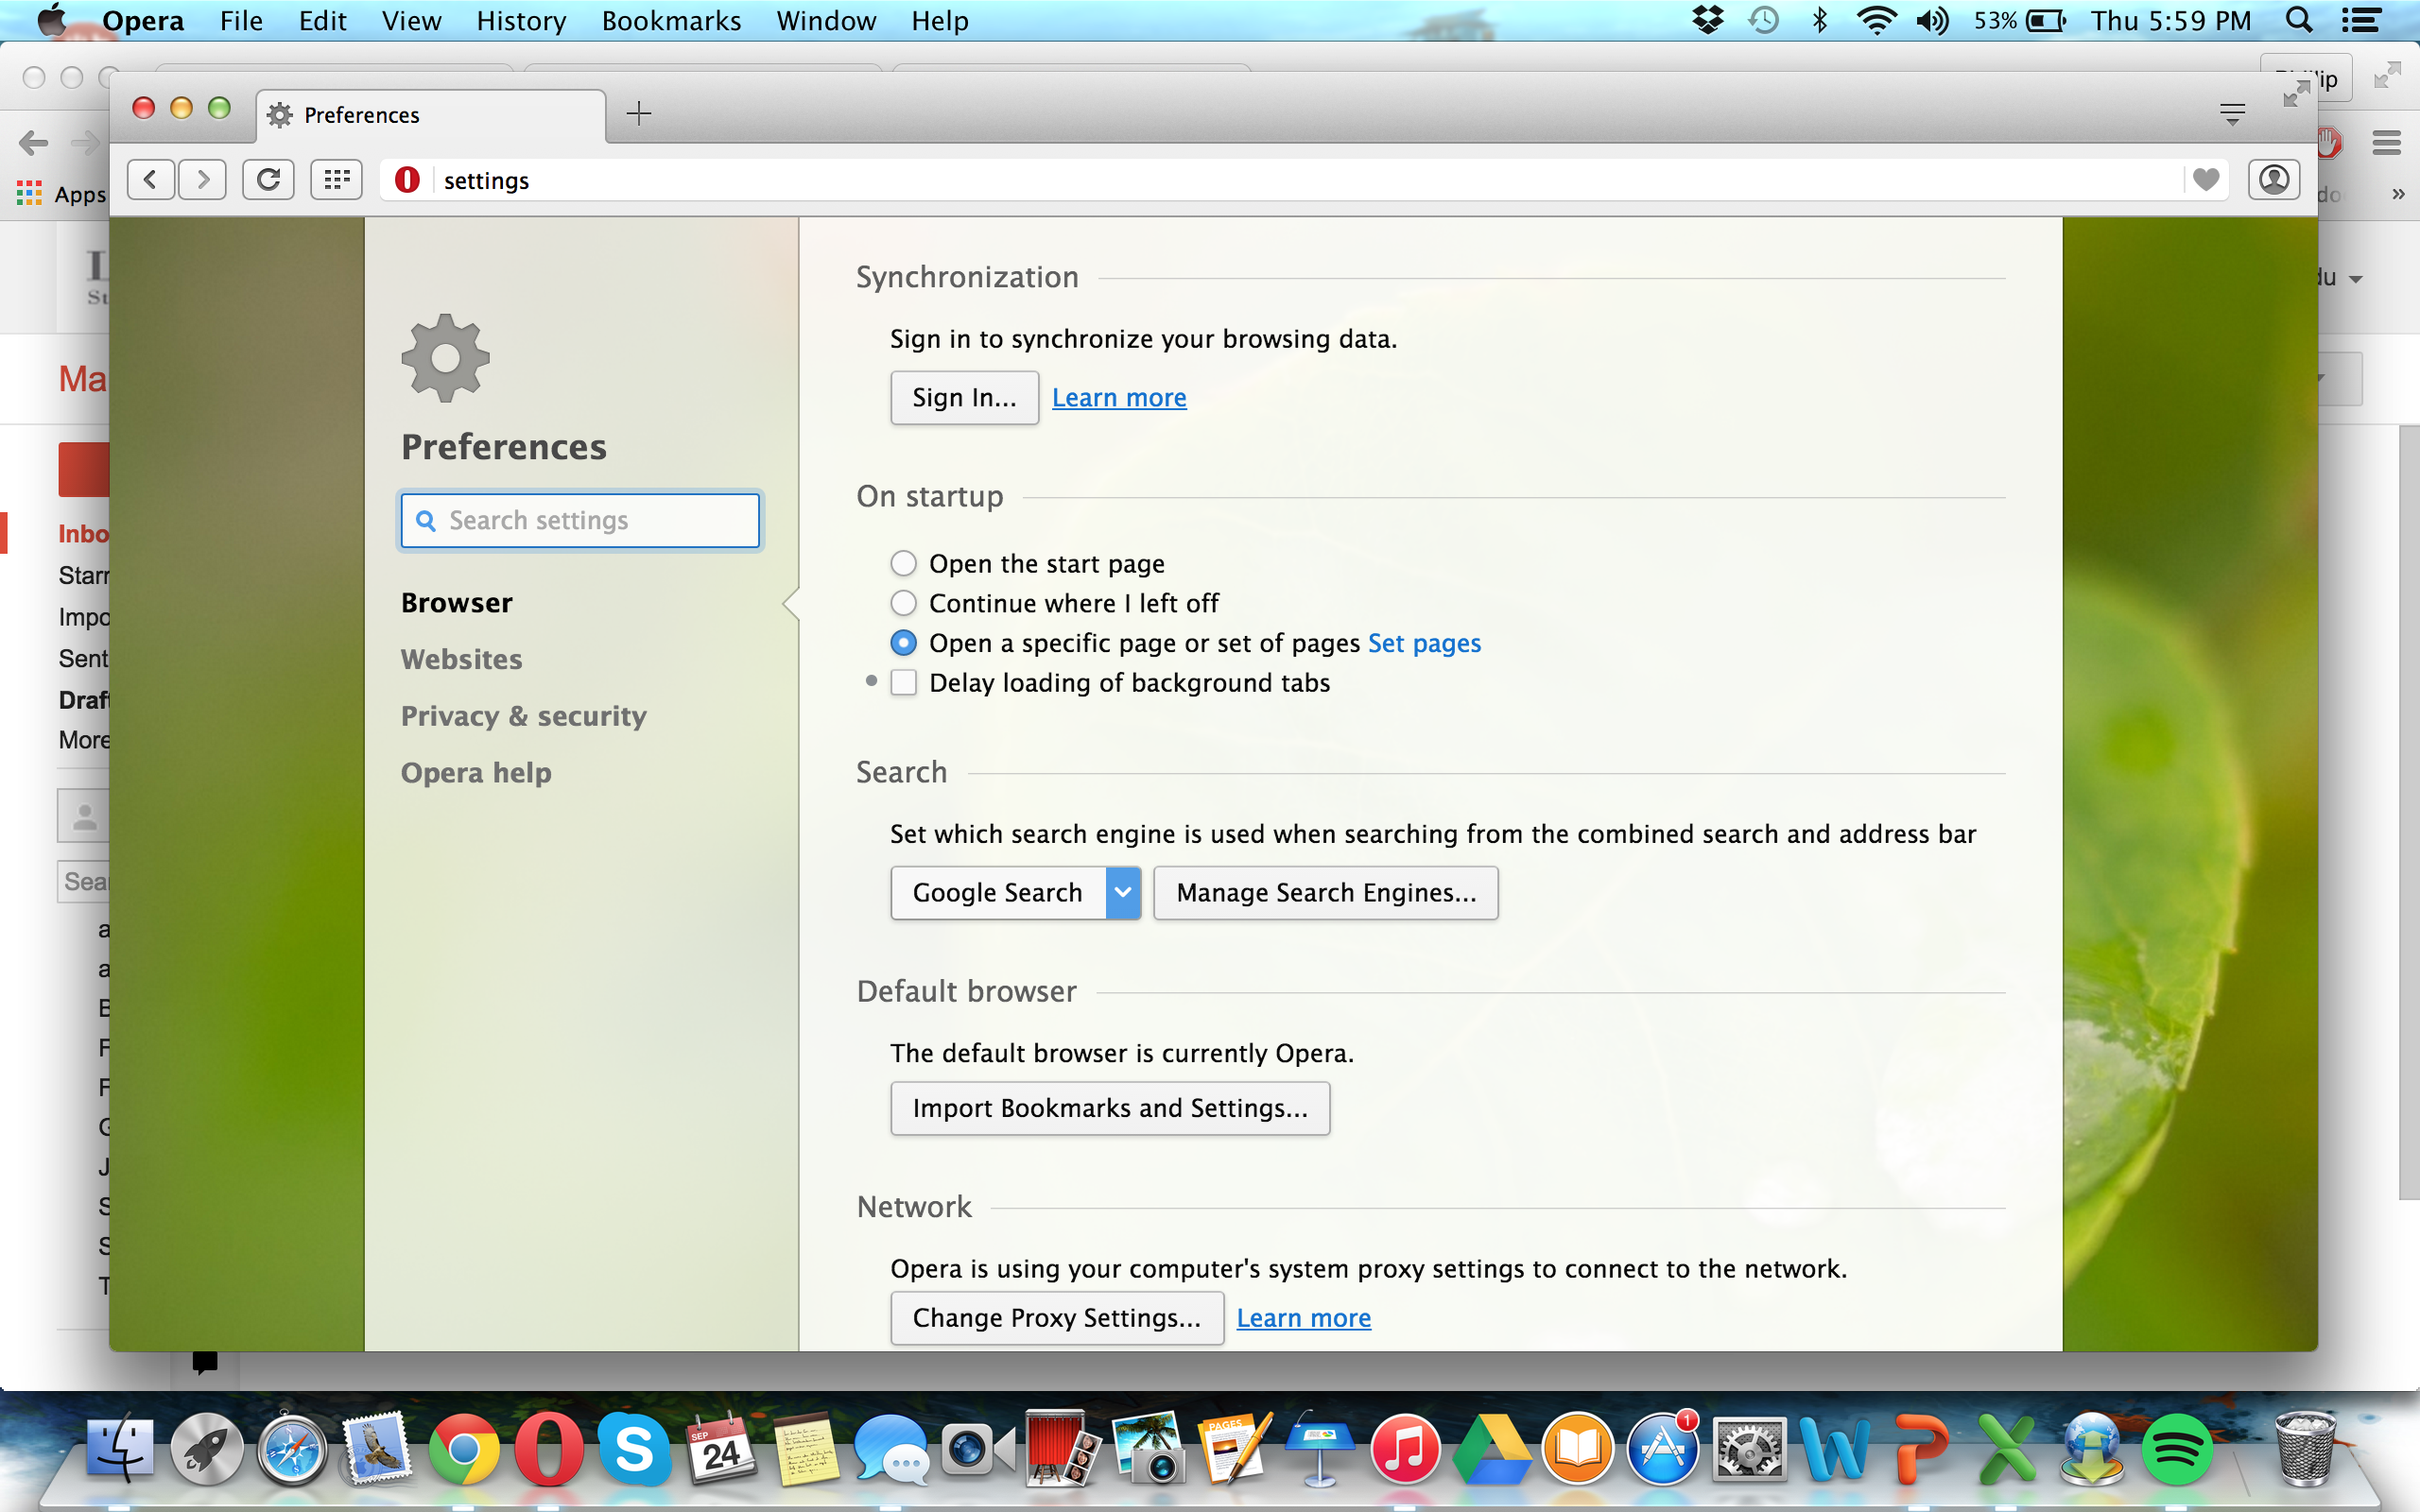
\includegraphics[width=1\textwidth]{Opera_Homepage.png}
\end{center}

\section{Conclusion}

\end{document}